%!TEX root = ../Thesis.tex

\section{Method}\label{sec:Method}

\subsection{Creating a Simulation}
Matlab was chosen as the platform to simulate and evaluate the program due to the ease of matrix manipulation and graphical interaction.
\subsubsection{Simulate Satellite Locations}
Using real ephemeris data for the GPS constellation, the location of all of the satellites were calculated, see Table \ref{Table: eph gps data}. The approximate reference location of the network of receivers was inputed into the program as longitude, latitude, height geocentric coordinate system. The satellite positions were transformed to the local tangent plane of the reference location in polar coordinates. The satellites that had an elevation of above 12$\deg$ were selected as potential visible satellites. This lower elevation limit was selected to minimised multipath effects that would likely occur at ground level \textcolor{red}{REF}. 
\begin{table}
\centering
\caption{Ephemeris data for GPS constellation}
\label{Table: eph gps data}
\begin{tabular}{|c|c|}
\hline
Orbital parameters & Value \\\hline
\end{tabular}
\end{table}

\subsubsection{True Location of Receivers}
The dispersion of receivers from $\alpha$ is a variable to the program. The actual displacement is calculated by multiplying the dispersion magnitude by a uniformly distributed random vector ranging from [0,1] in three dimensions for all remaining receivers in ECEF frame localised at $\alpha$. The positions were then transformed to the global ECEF frame.

\subsubsection{Calculation of Pseudorange}
In ECEF frame, the instantaneous distance between each visible satellite and each receiver was calculated. The errors were simulated by adding random distance proportional to error models in the literature to each individual satellite, see Table \ref{Table:mag errors}. The errors followed the structure in Eq
In the literature, the errors were expressed in meters which were converted to seconds.
\begin{eqnarray}
Error(seconds) = (Error)
\end{eqnarray}
\begin{table}
\centering
\caption{Magnitude of simulated errors}
\label{Table:mag errors}
\begin{tabular}{|c|c|}
\hline
Error Source & meters \\\hline
\end{tabular}
\end{table}

\subsubsection{Planar Algorithm}
The normal vector was


- what data is it using from receiver? psudorange, time\\

- what errors to include and how to incorporate into the simulation.\\
- how to include the different(asynchronous ) time received for all receivers-> is for the one receiver \\
- how extra receivers affects computational time/ accuracy\\
- how number of sats affect comp time/accuracy\\
- configuration of sats\\
- large multipath affects\\
- no receiver sees the same sat? - does it just output the relative difference between abs values? -> incorrect? just have it fail? not actually implementing, can control the environment\\
- distance of receivers apart\\
- configuration of receivers


- what data received and how to simulate misaligned timing between receivers\\
- what magnitude are the errors and how to simulate them\\
- simulate the errors individually (to see how each type affects the sim - convergence time and accuracy) and/or all errors at once


\subsection{Evaluation} % how to evaluate
The expected error due to the assumptions were outlined in Section XX. To evaluate the parallel plane assumption, two receivers were a set distance apart.


\paragraph{Dilution of Precision}
The dilution of precision (DOP) is a measure of how the geometry of the satellites affect the position measurement precision. It is used in GNSS to evaluate how much error there may be in a measurement. Figure \ref{Fig: GDOP abstract} shows two different configurations of satellites in the 2D circular solution case. With some error bounds as shown in B and C, the solution can lie anywhere in the green area. Due to the geometry configuration of the satellites in C, the area is considerably larger even though the error bounds on the signals are the same.

\begin{figure}
\centering
\caption{Geometric Dilution of Precision}
\label{Fig: GDOP abstract}
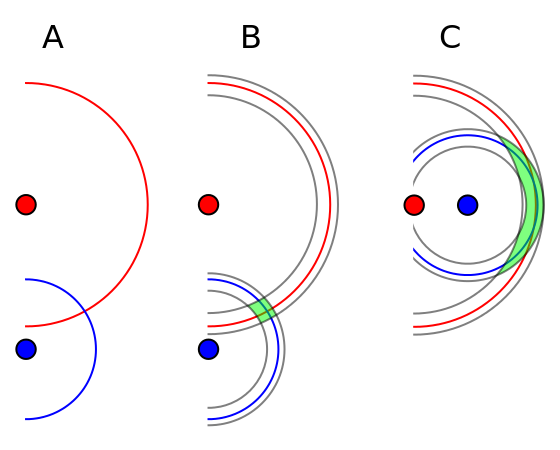
\includegraphics[width=0.7\linewidth]{ChapterExperiments/Figures/GDOP.png}
\end{figure}




- fake gps data\\
- how to simulate noise - what level SNR\\
- to calculate your own GPS location using the normal algorithm? - space 3 \\
- use real GPS locations? (and through time) -space 3\\
- vary number of satellites in view\\
- vary GDOP (good GDOP and bad)\\
- when receivers don't see the exact same satellites \\
- vary number of receivers \\
- simulate a multipath error and how does it account for it or how much error does it introduce\\

How to evaluate?:
- accuracy in relative space\\
- compare to just taking differences in absolute position \\
- between individual receivers and the total error in the whole system\\
- markov? error analysis -> cannot do precision without statistical analysis but isolate errors in x,y,z. how much worse is z than horizontal?\\
- computational time-> how does more receivers/satellites affect the comp time -> what time and space complexity?

